% !TEX root = ../../../../main/numb3rs_activities.tex
\newpage
\phantomsection
\addcontentsline{toc}{subsection}{108: Identity Crisis \label{ep108}}
\ep{108: Identity Crisis}
\setcounter{activity}{0}

A man accused of stock fraud is found garroted in his apartment and the crime is very similar to one committed a year ago. In this episode Charlie helps his brother to investigate the relation between the two murders in order to find out who is the perpetrator and to determine the innocence of the man arrested one year ago.


Below we will explain the illegal scheme used by the victim to gain money which is related to the concept of Geometric Progression or Geometric sequence.


% Pyramid 
\ltLarge{What is a Pyramid Scheme?}


A pyramid scheme is a fraudulent non-sustainable business model that --- as its name suggests --- takes the form of a pyramid. The scheme could be more complicated than the one presented here; however, the idea behind it is always the same: the people involved in the scheme must recruit others in order to recover their initial investment plus some profit, but the recruitment process is done only with the promise of earning money after recruiting others with no service or product in exchange.


\begin{ex}
There is one person on top of the pyramid. This person asks for a fixed amount of money, say \$1, to a second person with the promise that if he convinces two people to join and pay the entrance fee of \$1, he will get \$2 which would double up his/her initial investment. At this point the first two people have made \$1 dollar each without selling any product or giving any service. The other two people have to recruit two people each in order to double up their money. At this point, we are at the fourth level of the pyramid; where already $1+1+2+4=8$ people are involved in the scheme. As the pyramid gets bigger the amount of people increases really fast, at level n there will be $1 + 1 + 2 + \cdots + 2^{n-2}$ persons in the scheme and the bottom $2^{n-2}$ have to recruit $2^{n-1}$ new people in order to receive money. This is what makes the scheme fraudulent: since the amount of people involved increases \textbf{geometrically}, after a few levels the system will collapse because there are no more people to recruit and then the people at the bottom of the pyramid will loose their initial ``investment.''
\end{ex}

	\begin{figure}[H]
	\centering
	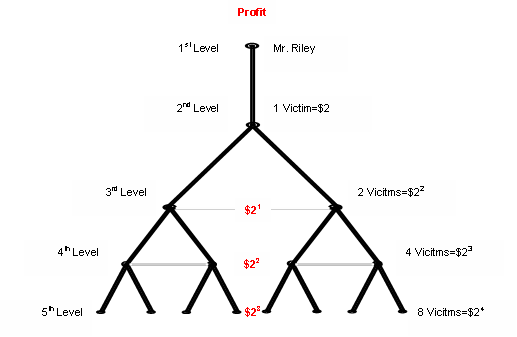
\includegraphics[width=0.80\textwidth]{../sections/seasons/season1/108/images/pyramid.png} 
	\end{figure}


\begin{ex}
The scheme presented above is very similar to the one Charlie explained to Don and Terry in the episode. In this case Mr. Riley started by taking \$2 out from one account, then he took \$2 out of other two accounts, he kept \$2 to himself and used the other \$2 to replace the money he had already taken, this corresponds to the third level of the pyramid. Then he took \$2 out of 4 accounts, he used \$4 to replace the money he had taken and kept the other \$4. He kept doing this so that at level $n$ of the pyramid he made $2^{n-2}$ dollars. The system crashed when he reached the 21st level of the pyramid, and at this point he obtained a profit of \$524.288 ($= \$2^{19}$) as mentioned in the show.
\end{ex}


% Geometric
\ltLarge{What is a Geometric Progression?}


A geometric progression is a sequence of numbers with the property that the quotient between any of the numbers and the previous one is a constant. This quotient is called the \textbf{ratio} of the progression. In mathematical notation a geometric progression or geometric sequence is a sequence of the form
	\[
	(a_n)_{n \geq 1} \text{ where, }a_n = ar^n \text{ for all } n.
	\]
$a$ is an arbitrary number and $r$ corresponds to the ratio of the progression. If the ratio of the progression is a number strictly greater than 1 as time evolves, i.e. as $n$ gets bigger, the terms of the progression become big really fast (this is the case in our examples above where $r=2$). If the ratio is equal to 1 the progression is constant, i.e. all its terms are actually the same. Finally, if the ratio of the progression is a positive number strictly less than 1 as time evolves the terms get smaller approaching 0. 


A concept that is closely related to the concept of Geometric Progression is the concept of \textbf{Geometric Series}. A geometric series corresponds to the sum (possibly infinite) of terms of a Geometric Progression. For instance, if you add the first $n$ terms of the geometric progression shown above then you will obtain
	\[
	ar + ar^2 + \cdots + ar^n = a \left( \dfrac{1 - r^{n+1}}{1 - r} -1 \right).
	\]
This equation is obtained from the following algebraic equation
	\[
	( 1 + r + \cdots + r^n)(1 - r) = 1 - r^{n+1}.
	\]
And if you add up all the terms of a geometric progression with ratio $r$, between 0 and 1, then you will obtain,
	\[
	\sum_{i=1}^\infty a_n = ar + ar^2 + \cdots + ar^n + \cdots = a \left(\dfrac{1}{1 - r} -1 \right).
	\]
This follows as a consequence of the formula above for n terms, and the fact that as $n$ gets bigger then $r^{n+1}$ approaches 0.


\activity{
\begin{enumerate}[(a)]
\item By using the formulas presented above calculate how many people are involved in the scheme of Example 1 above after 12 levels.
\item What is the total profit of Mr. Riley after the 21 levels of the pyramid? 
\end{enumerate}
}


\tangent{A different but similar kind of scheme is what is known as \textbf{Ponzi Scheme}. It is named after Charles Ponzi who after emigrating from Italy to the United States in 1903 earned a lot of money by implementing a short-term high return investment scheme, using the currency difference between the United States and foreign countries to buy and sell international mail coupons. In this scheme the actors interact with all the other people involved in the scheme which gives the scheme a non-pyramidal structure. Also the amount of people does not increase geometrically because reinvestment is allowed. This gives the scheme a longer life. However the scheme is fraudulent as well because it relies on the same principle as pyramid schemes: new money from the investors is used to pay off earlier investors until the whole scheme collapses.}


\begin{ex}[Doubling Strategy]
Geometric Progressions appear in numerous areas of study. Here we provide an example of their appearance in elementary financial theory through the key concept of \textbf{arbitrage}. We say that there exists arbitrage in a certain financial transaction if at least one of the parties involved obtains a risk-less profit after the transaction. For instance, consider the following coin toss game: an \emph{infinitely} rich gambler bets \$1 on tails. If the result after tossing the coin is tails he will double up his money obtaining \$2 and the game ends. If the result is heads he will lose his dollar but he has the chance to bet back again \$2. If in the second round the result is tails, then he will double up the \$2 getting \$4, obtaining a net profit of \$1 and the game will end, otherwise he will lose the \$2 cumulating a loss of $\$1+\$2=\$3$. However, since his wealth is infinite, in the later case he can bet \$4 in the third round. If he wins he will get \$8 and his net profit will be \$1, otherwise he will cumulate a total loss of $\$1+\$2+\$4=\$7$. The game keeps going in this direction indefinitely. The probability of the gambler winning \$1 by the end of the game is 1, and hence arbitrage exists. Notice that the amount of money the gambler has to bet in each round follows a geometric progression of ratio 2 and this is why he is assumed to have an unlimited liquidity. In order to avoid arbitrage, finance theory assumes limited liquidity.
\end{ex}


\activity{Suppose the game described above has not finished after 10 rounds. How much money has the gambler lost up to this point? How much money does he have to bet in the next round?}


% Fingerprint
\ltLarge{Fingerprint Analysis}


In this episode, Charlie also questions the terminology experts use in fingerprint recognition analysis. He criticizes the assumption often made in this area which states that there are no two people with the same fingerprint structure. However, Charlie explains that this may not be necessarily true because there is no way of knowing this in a deterministic way. He proposes that using probabilistic statements would be more appropriate - as is already the case in DNA match studies. Charlie's critic is founded on the following argument: world's population as of today is approximately 6.5 billion and each person's fingerprint structure contains a very high amount of information. This makes it almost impossible to file all this information in the data bases and demands the use of compressing methodologies in order to store such a high amount of information. In the compression of the fingerprint images only the main characteristics are taken into account and some of the details are not taken into consideration, which makes fingerprint recognition a probabilistic problem rather than a deterministic one. One of the algorithms the FBI has implemented for Fingerprint Compression uses Wavelet Analysis, a technique mentioned in \hyperref[ep107]{Episode 107} as well.